% !TeX spellcheck = en_US	

\documentclass[10pt,journal,compsoc]{IEEEtran}
\usepackage{graphicx}
\usepackage[ruled, linesnumbered]{algorithm2e}
\usepackage{url}
\usepackage{epstopdf}
\usepackage{indentfirst}
\usepackage[tight,footnotesize]{subfigure}
\usepackage{amsmath}
\usepackage{amssymb}
\usepackage{multirow}
\usepackage{color}
\usepackage{enumerate}

\newtheorem{theorem}{Theorem}[section]
\newtheorem{lemma}[theorem]{Lemma}
\newtheorem{observation}[theorem]{Observation}
\newtheorem{corollary}[theorem]{Corollary}
\newtheorem{formula}[theorem]{Formula}

% *** CITATION PACKAGES ***
\ifCLASSOPTIONcompsoc
\usepackage[nocompress]{cite}
\else
\usepackage{cite}
\fi

\begin{document}

\title{Building and Checking Suffix Array Using Induced Sorting Method}

\author{Yi~Wu,
	Ge~Nong,
	Wai~Hong~Chan,
	and~Bin~Lao
	\IEEEcompsocitemizethanks{
		\IEEEcompsocthanksitem Y. Wu, G. Nong (corresponding author) and B. Lao are with the Department of Computer Science, Sun Yat-sen University, Guangzhou 510275, China. E-mails: wu.yi.christian@gmail.com, issng@mail.sysu.edu.cn, Laobin@mail3.sysu.edu.cn.
		
		\IEEEcompsocthanksitem Wai Hong Chan (corresponding author) is with the Department of Mathematics and Information Technology, The Education University of Hong Kong, Hong Kong. E-mail: waihchan@ied.edu.hk.
}}% <-this % stops a space


\IEEEtitleabstractindextext{% 
\begin{abstract}

%The induced sorting~(IS) method has been applied to designing several disk-based suffix array~(SA) construction algorithms. Although these algorithms have better time and I/O complexities than the other alternatives, their current programs commonly suffer from a bottleneck due to the large disk space in need.

The induced sorting~(IS) method has been applied to designing efficient suffix array~(SA) construction algorithms on both internal and external memory models. In this paper, we propose two checking methods that enable any IS suffix sorters to check an SA when it is being built. The first method is capable of checking both suffix and LCP arrays for strings on constant alphabets, while the second method is specific for checking SA only but applicable to strings on both constant and integer alphabets. For performance analysis, we integrate the second checking method into the existing SA construction algorithm DSA-IS, where the design of DSA-IS is adapted by new substring sorting and naming methods for reducing its peak disk use to at most 14 times as input size. From our experimental results, the time, space and I/O consumptions for verification by our second method is negligible to that for construction by the adapted DSA-IS. This convinced that our checkers, together with the state-of-the-art IS suffix sorters, may constitute efficient solutions for building and checking SA at the same time.

\end{abstract}

% Note that keywords are not normally used for peerreview papers.
\begin{IEEEkeywords}
Suffix and LCP arrays, construction and verification, external memory.
\end{IEEEkeywords}}


% make the title area
\maketitle

\IEEEdisplaynontitleabstractindextext

\IEEEpeerreviewmaketitle

\section{Introduction}\label{sec:introduction}

The suffix array of any constant or integer string can be built in linear time and RAM space by SA-IS~\cite{Nong11}. The induced-sorting method has been also applied to designing fast external-memory SA construction algorithms eSAIS~\cite{Bingmann12}, DSA-IS~\cite{Nong15} and SAIS-PQ~\cite{Liu15}. These three disk-based variants have better time complexities than the other alternatives~(e.g., DC3~\cite{Dementiev2008a}, bwt-disk~\cite{Ferragina2012}, SAscan~\cite{Karkkainen2014} and pSAscan~\cite{Karkkainen2015}), but they all suffer from a bottleneck due to the large disk space in use. For example, when building SA encoded by 40-bit integers, the peak disk use for eSAIS, DSA-IS and SAIS-PQ are $24n$, $20n$ and $15n$, respectively. This situation changed due to the work presented in~\cite{Karkkainen2017}, which proposed a carefully engineered IS suffix sorter fSAIS that takes no more than $8n$ disk memory for any constant or integer string of size $n \le 2^{40}$~\cite{Karkkainen2017}. As reported, fSAIS reuses the substring/suffix sorting and naming methods of DSA-IS and SAIS-PQ, it achieves the remarkable space performance by means of a monotone priority queue for sorting fixed-size tuples and an I/O layer for allocating and deallocating disk space in a fine-grained way. The successful design of fSAIS shows a great potential for sharply decreasing the disk space requirements of the current programs for DSA-IS and SAIS-PQ. In this paper, we present our first attempt to improve DSA-IS by new substring sorting and naming methods. From the experiments, our program for the adapted algorithm DSA-IS+ takes $12n$ disk space in average and runs as fast as eSAIS on various real-world datasets. We will demonstrate that this program can be further improved using the optimization technique for implementing fSAIS.

To avoid computation errors caused by implementation bugs and/or hardware malfunctions, an SA should be checked to ensure its correctness after construction. Currently, the software packages for DC3 and eSAIS provide users a checker based on the method proposed in~\cite{Dementiev2008a}, which performs two disk sorts for $\mathcal{O}(n)$ fixed-size tuples with an integer key. When running in external memory, this checker takes one-third as much time and I/O consumptions as the programs for DSA-IS and eSAIS, it also requires nearly the same disk space as the two SA builders. Against the background, we propose two checking methods that enable any IS suffix sorting algorithm to build and check SA at the same time. In comparison with the previous checking method, they are rather lightweight in terms of time, space and I/O volume. It should be noticed that these two methods are designed for different situations. In brief, the first method can check both suffix and LCP arrays, but it is specific for strings on constant alphabets. The second method can be applied to strings on constant and integer alphabets, but it can check SA only. As will be seen in our experiments, the consumption for checking by our second method is negligible compared with that for building by DSA-IS+.

The rest of this paper is organized as follows. Section~\ref{sec:builder} describes the framework of IS suffix sorting algorithms and the idea of new substring sorting and naming methods, Section~\ref{sec:checkers} the designs of two checking methods, Sections~\ref{sec:experiments} the experimental results, and Section~\ref{sec:conclusion} the concluding remarks.

\section{Builder}~\label{sec:builder}

\subsection{Preliminaries}

Consider a string $x[0,n)$ drawn from a full-ordered alphabet $\Sigma$. The ending character $x[n - 1]$ is supposed to be unique and lexicographically smaller than any others in $x$. For convenience, we denote by ${\sf suf}(i)$ the suffix running from $x[i]$ to the ending character and ${\sf sub}(i,j)$ the substring running from $x[i]$ to $x[j]$, respectively. The following notations are also used in our presentation.

{\em Character/substring/suffix classification.} Characters in $x$ are classified into two categories: L-type and S-type. We say $x[i]$ is S-type if (1) $i = n - 1$ or (2) $x[i] = x[i + 1]$ and $x[i + 1]$ is S-type; otherwise $x[i]$ is L-type. Furthermore, if $x[i]$ and $x[i - 1]$ are respectively S-type/L-type and L-type/S-type, then $x[i]$ is also called S*-type/L*-type. An array $t$ records the type of all the characters in $x$, $t[i]$ is set to $1$ or $0$ if $x[i]$ is S-type or L-type, respectively. Each substring/suffix is of the same type as its heading character. In this paper, we only consider the substrings ending with an S*-type character.

{\em Predecessor and successor.} Given two characters $x[i]$ and $x[i + 1]$, $x[i]$ is the predecessor of $x[i + 1]$ and $x[i + 1]$ is the successor of $x[i]$. Accordingly, we define the predecessor-successor relationship between two suffixes or substrings starting with neighboring characters.

{\em Reduced string.} Split $x$ into multiple substrings such that each substring only contains two S*-type characters at the starting and ending positions. Assign each substring a name and replace them with their names to produce a reduced string $x_1$, where the name indicates the lexical order of the corresponding substring among all.


{\em Suffix array.} The suffix array $sa$ indicates the lexicographical order of all the suffixes in $x$, where $sa[i]$ records the starting position of the $(i + 1)$-th smallest suffix. We also define the SA for $x_1$ by $sa_1$.

\subsection{Introduction to IS Suffix Sorting Algorithms} \label{subsec:improvement}

% Algorithm
\begin{algorithm}
	\SetAlgoNoLine
	\KwIn{$x$}
	\KwOut{$sa$}
	
	/* Reduction Phase */ \\
	Sort S*-type substrings by the IS method.
	
	Name the sorted S*-type substrings to produce $x_1$.
	
	~\\
	
	/* Check Recursion Condition */ \\	
	\If{exist two equal characters in $x_1$}{
		
		
		Recursively call the reduction phase on $x_1$.
	}
	
	~\\
	
	/* Induction Phase */ \\
	Sort suffixes by the IS method.
	
	
	\caption{The general framework for an IS suffix sorting algorithm.}
	
	\label{alg:1}
\end{algorithm}

As shown in Algorithm~\ref{alg:1}, an IS suffix sorting algorithm first performs a reduction phase to produce the reduced string $x_1$. If there exist two equal characters in $x_1$, then it recursively calls the reduction phase with $x_1$ as input; otherwise, all the S*-type suffixes in $x$ are already sorted and it performs an induction phase to produce $sa$ from these sorted suffixes. According to the IS principle, the order of two substrings/suffixes is determined by comparing their heading characters and successors in sequence during the execution of reduction/induction phase. Notice that this key operation takes multiple random accesses to $x$ and $sa$. It can be done very quickly if both $x$ and $sa$ are wholly loaded into RAM; otherwise, each access may take an individual I/O operation to external memory and thus becomes the bottleneck. 

To amortize the I/O overhead, eSAIS, DSA-IS and SAIS-PQ use different methods to obtain heading characters in a disk-friendly way. Particularly, DSA-IS first divides $x$ into multiple blocks and calls SA-IS to sort suffixes in each block at the beginning of induction phase, where the heading characters in need are written to external memory in their access order. Then, it organizes the sorted suffixes in a priority queue and visits them sequentially to induce the order of their predecessors following the IS principle. Because the required heading characters was already stored on disks, they can be read into RAM by sequential I/O operations when needed. This technique is also applied to sorting substrings during the reduction phase. Afterward, a naming process is conducted to check equality of lexicographically neighboring substrings for producing the reduced string $x_1$. To do this, DSA-IS maintains a copy for each substring in external memory and arranges them in their sorted order. As can be seen in Section~\ref{sec:experiments}, our program for DSA-IS requires less disk space than that for eSAIS, but it runs slower than the latter due to the large I/O volume for sorting and naming S*-type substrings. 


\subsection{Improvements on DSA-IS}

We first describe a new method for sorting S*-type substrings during the reduction phase. Given an integer value $D$, all the S*-type substrings are classified into long and short categories with respect to whether or not they contain more than $D$ characters. Our sorting method executes the following three steps in sequence after splitting $x$ into blocks $\{b_1, b_2, ...\}$. 

\begin{enumerate}[S1]
	\item Sort S*-type substrings in each block by calling the reduction phase of SA-IS. Copy the short substrings and store them on the disk in their sorted order. Copy the heading characters needed for sorting long substrings and store them on the disk in their access order.~\label{sort_and_name_method:1}
	
	\item Sort long S*-type substrings by the same way of DSA-IS. Copy the leftmost $D$ characters of the long substrings and store them on the disk in their sorted order.~\label{sort_and_name_method:2}
	
	\item Merge short and long S*-type substrings by a multi-way sorter.~\label{sort_and_name_method:3}
\end{enumerate}

Assume the number of blocks is $k$, S\ref{sort_and_name_method:1} copies the sorted short substrings in $b_i$ to an external memory vector $vs_i$ and S\ref{sort_and_name_method:2} copies the sorted long substrings to an external memory vector $vl$. Then, S\ref{sort_and_name_method:3} uses a sorter to merge these partial results, where the sorter maintains a minimal heap in RAM to determine the current smallest substring in $vs_1, vs_2, ..., vs_k$ and $vl$. For any two substrings in the heap, their lexicographical order can be determined in $\mathcal{O}(D)$ time by literally comparing their characters from left to right. This sorting method achieves a good performance when most of the S*-type substrings are short. This makes it feasible in practice because the average length of S*-type substrings in real-world datasets are typically small.

Next, we describe how to name S*-type substrings at the same time when they are being sorted. Given two S*-type substrings successively popped from the minimal heap, we make a literal comparison of them to check their equality if they are both short; otherwise, we use the naming method of SAIS-PQ to determine their equality in S\ref{sort_and_name_method:2}. Specifically,
substrings are sorted by comparing their heading characters and the names of their sorted successors in S\ref{sort_and_name_method:2}, where two substrings are of the same name if and only if their heading characters and the names of their successors are both equal. By recording the names of long S*-type substrings in their sorted order, it takes constant time to check equality of two lexicographically neighboring long substrings in S\ref{sort_and_name_method:3}.

\subsection{Discussion} \label{subsec:further_discussion}

Section~\ref{sec:experiments} shows that, by using the new substring sorting and naming methods, our program for the enhanced  DSA-IS has an advantage over that for eSAIS in terms of space and I/O volume, but its average peak disk use is still higher than that for fSAIS by around $5n$. This is mainly due to the use of external-memory containers (vectors, sorters and priority queues) provided by the STXXL library~\cite{Dementiev2007}. More specifically, the STXXL's containers fail to free the disk space for saving temporary data immediately after they are no longer to use. This implementation issue can be solved by storing temporary data into multiple files and deleting each file when it is obsolete. In this way, our program can be further improved to achieve a space performance similar to that for fSAIS.

\section{Checkers}~\label{sec:checkers}

\subsection{Prior Art} \label{sec:checkers:prior_art}
The widespread software packages for DC3 and eSAIS provide users a checker to perform verification. Theorem~\ref{theorem:1} gives the main idea behind this checker. 

\begin{theorem} \label{theorem:1}
	$sa[0, n)$ is the SA for $x[0, n)$ if and only if the following conditions are satisfied:\\
	(1) $sa$ is a permutation of $[0, n)$. \\	
	(2) ${\sf r_i < r_j} \Leftrightarrow (x[i], r_{i + 1}) < (x[i], r_{j + 1})$ for $ i, j \in [0, n)$ and $i\ne j$, where $r_i$ and $r_j$ indicates the relative order of ${\sf suf}(i)$ and ${\sf suf}(j)$ among all the suffixes, respectively. \\
\end{theorem}

\begin{IEEEproof}
	The proof is available in~\cite{Dementiev2008a}.
\end{IEEEproof}

This checker performs two passes of integer sorts and each sort involves $n$ fixed-size tuples. When implemented in external memory, it requires large disk space and consumes high I/O volume, resulting in a non-negligible checking overhead. As will be seen in Section~\ref{sec:experiments}, the peak disk use for checking an SA encoded by 40-bit integers is around $21n$, while the I/O volume is no less than $50n$. In this section, we describe two lightweight SA checking methods based on the IS principle. Both of them can be seamlessly integrated into any IS suffix sorting algorithm to build and check SA simultaneously.  

\subsection{Method A} \label{sec:checkers:method_a}

\subsubsection{Preliminaries} \label{sec:checkers:method_a:preliminaries}

{\em LCP array.} The LCP array for $sa$, denoted by $lcp$, satisfies that $lcp[0] = 0$ and $lcp[i] = \ell$ for $i \in [1, n)$, where $\ell$ is the length of the longest common prefix of ${\sf suf}(sa[i])$ and ${\sf suf}(sa[i - 1])$.

{\em Suffix and LCP buckets.} All the suffixes in $sa$ are naturally partitioned into multiple buckets. Each bucket contains suffixes starting with a same character and occupies a contiguous interval of $sa$. For example, ${\sf sa\_bkt}(c_0)$ gathers all the suffixes starting with $c_0$. This bucket can be further partitioned into two parts, where the left and right parts only contain the L-type and S-type suffixes, respectively. For short, we denote the left and right parts by ${\sf sa\_bkt_L}(c_0)$ and ${\sf sa\_bkt_S}(c_0)$, respectively. Accordingly, $lcp$ can be also partitioned into multiple buckets and ${\sf lcp\_bkt}(c_0)$ records the LCP-values of suffixes in ${\sf sa\_bkt}(c_0)$. Similarly, we define ${\sf lcp\_bkt_L}(c_0)$ and ${\sf lcp\_bkt_S}(c_0)$ for ${\sf sa\_bkt_L}(c_0)$ and ${\sf sa\_bkt_S}(c_0)$, respectively.

{\em Suffix and LCP arrays for S*-type suffixes.} Let $n_1 = \|x_1\|$, we use $sa^*[0, n_1)$ and $lcp^*[0, n_1)$ to denote the suffix and LCP arrays for S*-type suffixes, respectively. The $i$-th element in $sa^*$ records the starting position of the $(i + 1)$-th smallest S*-type substring, while the $i$-th element in $lcp^*[i]$ records the LCP-value of ${\sf suf}(sa^*[i])$ and ${\sf suf}(sa^*[i - 1])$.

\subsubsection{Idea} \label{sec:checkers:method_a:idea}

During the induction phase, SA-IS first computes $sa^*$ by sorting the starting positions of all the S*-type suffixes with their ranks indicated by $sa_1$ and then induces $sa$ from $sa^*$ by S\ref{induction_phase:1}'-S\ref{induction_phase:3}'.

\begin{enumerate}[S1']
	
	\item Scan $sa^*$ rightward with $i$ decreasing from $n_1 - 1$ to $0$. For each scanned item $sa^*[i]$, insert it into the rightmost empty position of ${\sf sa\_bkt_S}(x[sa^*[i]])$. \label{induction_phase:1}
	
	\item Scan $sa$ rightward with $i$ increasing from $0$ to $n - 1$. For each scanned non-empty item $sa[i]$, insert $sa[i] - 1$ into the leftmost empty position of ${\sf sa\_bkt_L}(x[sa[i] - 1])$ if $t[sa[i] - 1] = 0$.\label{induction_phase:2}
	
	\item Scan $sa$ leftward with $i$ decreasing from $n - 1$ to $0$. For each scanned non-empty item $sa[i]$, insert $sa[i] - 1$ into the rightmost empty position of ${\sf sa\_bkt_S}(x[sa[i] - 1])$ if $t[sa[i] - 1] = 1$.\label{induction_phase:3}
	
\end{enumerate}

An example of the above inducing process is given in Fig.~\ref{fig:example1}. In line 6, we find the end of each bucket and insert the sorted S*-type suffixes into the corresponding buckets. Then, we find the head of each bucket (marked by the symbol $\wedge$) and scan $sa$ rightward for inducing the order of L-type suffixes. In lines 8-9, we check $\sf suf(14)$ (marked by the symbol $@$) and find its predecessor ${\sf suf(13)}$ is L-type, thus we put ${\sf suf(13)}$ into the current leftmost empty position in ${\sf sa\_bkt_L}(i)$. To step through $sa$ in this way, we get all the L-type suffixes sorted in line 17. After that, we find the end of each bucket and scan $sa$ leftward for inducing the order of S-type suffixes in lines 18-29. When scanning $sa[14]$, we see $x[3]$ is S-type and thus put ${\sf suf(3)}$ into the current rightmost empty position in ${\sf sa\_bkt_S}(i)$. Following the same, we get all the S-type suffixes sorted in line 29.


\begin{figure}[t]
	\centering
	
	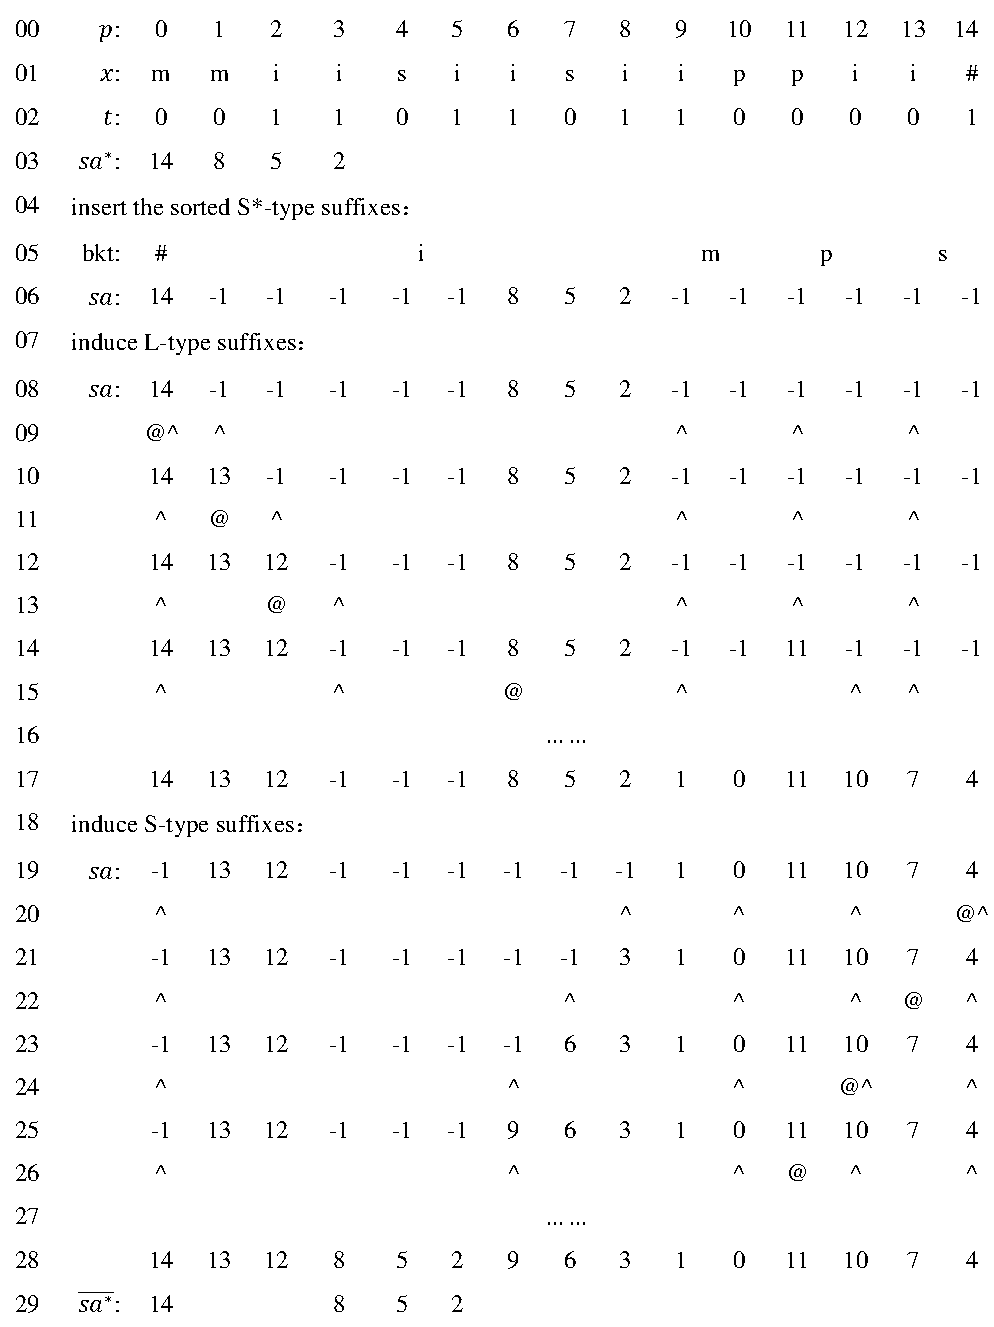
\includegraphics[width = 1\columnwidth]{example.pdf}
	
	\caption{An example for inducing $sa$ from $sa^*$.}
	
	\label{fig:example1}
	
\end{figure}

As stated below, S\ref{induction_phase:1}'-S\ref{induction_phase:3}' also constitute the sufficient and necessary conditions for a correct $sa$.

\begin{lemma} \label{lemma:3}
	For any IS suffix sorting algorithm, its output $sa[0, n)$ is the SA for the input string $x[0, n)$ if and only if the following conditions are satisfied: \\ 
	(1) $sa^*$ is correct. \\
	(2) $sa[i]$ is equal to the value calculated by SS\ref{induction_phase:1}-SS\ref{induction_phase:3}. \\
	
\end{lemma}

Suppose $sa^*$ is correct\footnote{The correctness of $sa^*$ can be checked by a sparse SA checker, such as~\cite{wu2017}. The checking processes for $sa^*$ and $sa$ can be executed in parallel.}, this lemma suggests a method to check $sa$ when it is induced from $sa^*$ during the induction phase. Specifically, in S\ref{induction_phase:2}' and S\ref{induction_phase:3}', each item induced into $sa$ will be scanned later to induce the order of its predecessor. If the induced and scanned values for each item are equal, then $sa$ is correct according to Lemma~\ref{lemma:3}. The problem to be solved here is that when an item is induced into a bucket, its value in $sa$ will not be scanned at once. Our solution for this is to integrate the building and checking processes into a whole, by ensuring the sequence of items induced into a bucket is identical to that scanned later. For the purpose, we increasingly compute the fingerprints of both sequences and check their equality at the end of the induction phase. If the two fingerprints for each bucket are equal, then the second condition of Lemma~\ref{lemma:3} will be seen with a high probability. As a result, $sa$ can be built and probabilistically checked at the same time, for this we have Corollary~\ref{corollary:1}.

\begin{corollary} \label{corollary:1}
	$sa[0, n)$ is the SA for the input string $x[0, n)$ with a high probability if the following conditions are satisfied for all $c \in \Sigma$: \\
	(1) $sa^*$ is correct.\\
	(2) The fingerprints of ${\sf sa_{I1}}(c)$ and ${\sf sa_{S1}}(c)$ are equal. \\
	(3) The fingerprints of ${\sf sa_{I2}}(c)$ and ${\sf sa_{S2}}(c)$ are equal. \\
	
\end{corollary}

Notice that ${\sf sa_{I1}}(c)$ and ${\sf sa_{I2}}(c)$ are two sequences respectively induced into ${\sf sa\_bkt_L}$ and ${\sf sa\_bkt_S}$, while ${\sf sa_{S1}}(c)$ and ${\sf sa_{S2}}(c)$ are two sequences respectively scanned from ${\sf sa\_bkt_L}$ and ${\sf sa\_bkt_S}$. 

\subsection{Method B}\label{sec:checkers:method_b}

We introduce Lemma~\ref{lemma:1} before the presentation of Method B. This statement has been applied to deriving Theorem~\ref{theorem:1} for comparing two suffixes given the order of their successors already known.

\begin{lemma} \label{lemma:1}
	For $i, j \in [0, n)$ and $i \ne j$, ${\sf suf}(i) < {\sf suf}(j) \Leftrightarrow (x[i], {\sf suf}(i + 1)) < (x[j], {\sf suf}(j + 1))$.
\end{lemma}

Below we describe the idea of Method B and prove its correctness using Lemma~\ref{lemma:1} and Theorem~\ref{theorem:1}, where $\overline{sa^*}$ is retrieved from $sa$ and it records the starting positions of all the S*-type suffixes in their sorted order.

\begin{theorem} \label{theorem:2}
	For any IS suffix sorting algorithm, its output $sa[0, n)$ is the SA for the input string $x[0, n)$ if and only if the following conditions are satisfied for all $i \in [0, n_1)$: \\
	(1) $sa^*[i]$ is the starting position of an S*-type suffix and it differs from any other items in $sa^*$. \\
	(2) $sa^*[i] = \overline{sa^*}[i]$. \\
\end{theorem}

\begin{IEEEproof}
	We only prove the sufficiency as the necessity is clear.
	
	Suppose $sa$ is not a permutation of $[0, n)$. Without loss of generality, let $i \ne j$ and $sa[i] = sa[j]$, then $u \ne v$ and $sa[u] = sa[v]$ according Theorem~\ref{theorem:1}, where ${\sf suf}(sa[u])$ and ${\sf suf}(sa[v])$ are the successors of ${\sf suf}(sa[i])$ and ${\sf suf}(sa[j])$, respectively. By recursively replacing $(i, j)$ with $(u, v)$, we can find two items $sa[i_0]$ and $sa[j_0]$ storing the starting position of the same S*-type suffix, indicating that $sa^*$ contains duplicate items. This violates condition (1) of Theorem~\ref{theorem:2}.
	
	Suppose $i < j$ and ${\sf suf}(sa[i]) > {\sf suf}(sa[j])$. If $x[sa[i]] < x[sa[j]]$, then ${\sf suf}(sa[i]) < {\sf suf}(sa[j])$ according to Lemma~\ref{lemma:1}; otherwise, if $x[sa[i]] > x[sa[j]]$, then $i > j$ according to Theorem~\ref{theorem:1}. Both two conditions lead to a contradiction. Therefore, we must have $x[sa[i]] = x[sa[j]]$. If so, then $u < v$ and ${\sf suf}(u) > {\sf suf}(v)$, where ${\sf suf}(sa[u])$ and ${\sf suf}(sa[v])$ are the successors of ${\sf suf}(sa[i])$ and ${\sf suf}(sa[j])$, respectively. By recursively replacing $(i, j)$ with $(u, v)$, we can find two elements $sa[i_0]$ and $sa[j_0]$ such that at least one stores the starting position of an S*-type suffix. We continue the proof following one of the three cases below:
	\begin{enumerate}[(1)]
	\item $x[sa[i_0]]$ is S*-type and $x[sa[j_0]]$ is L-type. In this case, $x[sa[i_0] + 1] > x[sa[j_0] + 1]$. Therefore, $u_0 > v_0$ according to Theorem~\ref{theorem:1}. This indicates that $(x[sa[i_0]], u_0) > (x[sa[j_0]], v_0)$ and thus $i_0 > j_0$ according to Theorem~\ref{theorem:1}. This leads to a contradiction.
	\item $x[sa[i_0]]$ is L-type and $x[sa[j_0]]$ is S*-type. In this case, $x[sa[i_0] + 1] < x[sa[j_0] + 1]$. Therefore, ${\sf suf}(sa[u_0]) < {\sf suf}(sa[v_0])$ according to Lemma~\ref{lemma:1}. This indicates that $(x[sa[i_0]], {\sf suf}(sa[u_0])) < (x[sa[j_0]], {\sf suf}(sa[v_0])$ and thus ${\sf suf}(sa[i_0]) < {\sf suf}(sa[j_0])$ according to Lemma~\ref{lemma:1}. This leads to a contradiction.
	\item $x[sa[i_0]]$ and $x[sa[j_0]]$ are both S*-type. Let $(i_0, j_0)$ be the pair that maximize $sa[i_0] + sa[j_0]$ such that $i_0 < j_0$ and ${\sf suf}(sa[i_0]) > {\sf suf}(sa[j_0])$, then $u_0 > v_0$ and ${\sf suf}(sa[u_0]) > {\sf suf}(sa[v_0])$. \footnote{Notice that $(u_0, v_0)$ must exist because the sentinel is a size-one S*-type substring smaller than others.} Because $x[i_0, u_0) = x[j_0, v_0)$, there must be $i_0 > j_0$ according to Theorem~\ref{theorem:1}, thus $sa^*$ and $\overline{sa^*}$ differ from each other. This violates condition (2) of Theorem~\ref{theorem:2}.
	\end{enumerate}

\end{IEEEproof}

The first condition of Theorem~\ref{theorem:2} is naturally satisfied when computing $sa^*$ from $sa_1$. A naive method for checking the second condition is to keep a copy of $\overline{sa^*}$ when computing $sa$ from $sa^*$ and compare it with $sa^*$ afterward. This takes linear time, space and I/O overhead. We prefer to check equality of them by comparing their fingerprints, which can be calculated during the scan of these arrays in S\ref{induction_phase:1}' and S\ref{induction_phase:3}'. 

\begin{corollary} \label{corollary:2}
	$sa[0, n)$ is the SA for the input string $x[0, n)$ with a high probability if the following conditions are satisfied for all $i \in [0, n_1)$: \\
	(1) $sa^*[i]$ is the starting position of an S*-type suffix and it differs from any other items in $sa^*$. \\
	(2) The fingerprints of $sa^*$ and $\overline{sa^*}$ are equal. \\
\end{corollary}

In Fig.~\ref{fig:example1}, both $sa^*$ and $\overline{sa^*}$ contain 4 items $14, 8, 5, 2$ arranged in the same order. By using the fingerprinting function introduced in the next subsection, the fingerprints can be calculated in linear time using constant space. 

\subsection{Discussion}

\begin{figure}[htbp!]
	\centering
	
	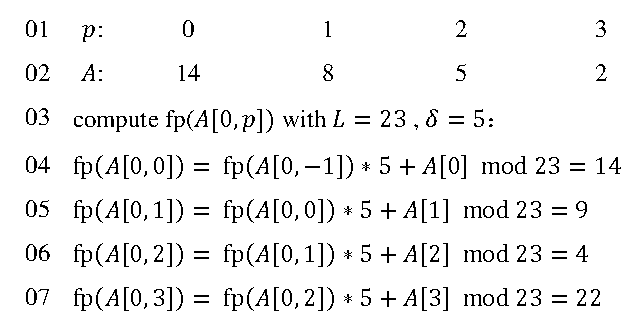
\includegraphics[width = 0.9\columnwidth]{example2.pdf}
	
	\caption{An example for calculating fingerprints by Karp-Rabin fingerprinting function.}
	
	\label{fig:example2}
	
\end{figure}

Methods A and B check equality of two integer arrays by comparing their fingerprints. In our programs, we choose to use the Karp-Rabin fingerprinting function to compute the fingerprints in need. As depicted in Fig.~\ref{fig:example2}, the fingerprint of $A$ is calculated according to Formulas~\ref{formula:1}-\ref{formula:2}, where $L$ is a prime and $\delta$ is an integer randomly chosen from $[1, L)$. It should be noticed that two equal arrays must have an identical fingerprint, but the inverse is not always true. Fortunately, the probability of a false match can be reduced to a negligible level if $L$ is set to a large value. 

\begin{formula} \label{formula:1}${\sf fp}(A[0, -1]) = 0$. 
\end{formula}

\begin{formula} \label{formula:2}${\sf fp}(A[0, i]) = {\sf fp}(A[0, i - 1]) \cdot {\delta} + A[i]\mod L$ for $i \ge 0$.
\end{formula}

We also point out that Method A can check $lcp$ when it is being built from $lcp^*$ following the IS principle~\cite{Fischer11}. This is done by comparing the sequence of items induced into an $lcp$ bucket with that scanned from the same bucket. If the two sequences of each bucket are equal, then $lcp$ is correctly the LCP array for $sa$.

\section{Experiments} \label{sec:experiments}

For implementation simplicity, we engineer DSA-IS and DSA-IS+ by the STXXL's containers~(vector, sorter, priority queue and stream). The experimental platform is a desktop computer equipped with an Intel Xeon E3-1220 V2 CPU, 4GiB RAM and 500GiB HD. All the programs are complied by gcc/g++ 4.8.4 with -O3 options under Ubuntu 14.04 64-bit operating system. In our experiments, three performance metrics are investigated for the programs running on the corpora listed in Table~\ref{tbl:corpora}, where each metric is measured as a mean of two runs.

\begin{itemize}
	\item construction time~(CT): the running time, in units of microseconds per character.
	\item peak disk use~(PDU): the maximum disk space requirement, in units of bytes per character.
	\item I/O volume~(IOV): as the term suggests, in units of bytes per character.
\end{itemize}

%Table
\renewcommand\arraystretch{1.3}
\begin{table}[!h]
	\caption{Corpus, $n$ in Gi, 1 byte per character} 
	\label{tbl:corpora}
	\centering
	\begin{tabular}{|l|c|c|p{5cm}|}
		\hline
		Corpora & \multicolumn{1}{c|}{$n$} & \multicolumn{1}{c|}{$\|\Sigma\|$} & Description \\\hline
		guten & 22.5 & 256 & Gutenberg, at \url{http://algo2.iti.kit.edu/bingmann/esais-corpus}.\\\hline 				
		enwiki & 74.7 & 256 & Enwiki, at \url{https://dumps.wikimedia.org/enwiki}, dated as 16/05/01. \\\hline	
		proteins & 1.1 & 27 & Swissprot database, at \url{http://pizzachili.dcc.uchile.cl/texts/protein}, dated as 06/12/15. \\\hline
		uniprot & 2.5 & 96 & UniProt Knowledgebase release 4.0, at \url{ftp://ftp.expasy.org/databases/.../complete}, dated as 16/05/11. \\\hline
	\end{tabular}
\end{table}

\subsection{Building Performance}

\begin{figure*}[t]
	\centering
	\subfigure[enwiki]{
		\begin{minipage}[b]{0.45\textwidth}
			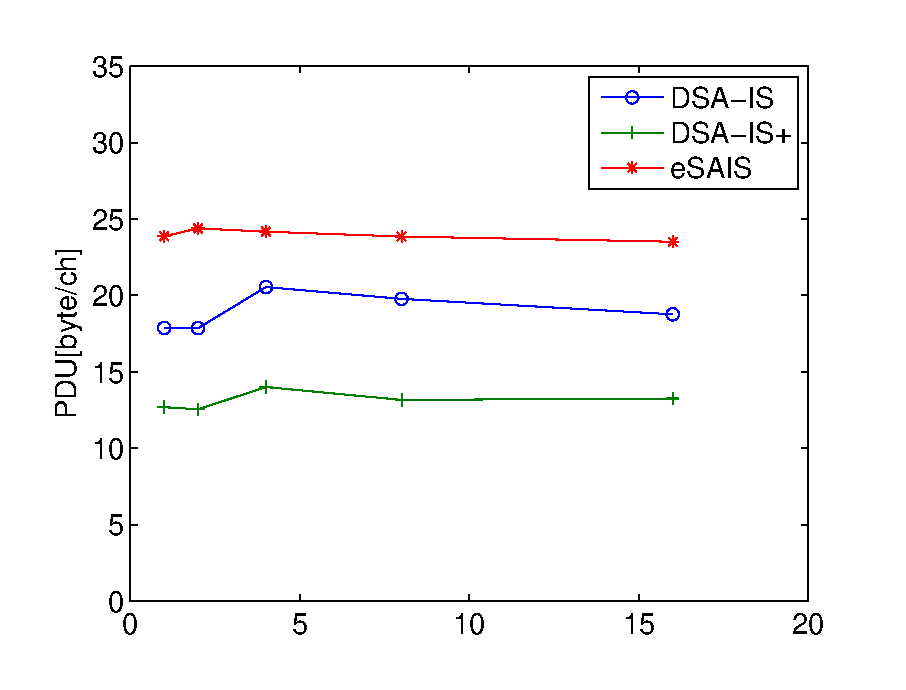
\includegraphics[width=1\textwidth]{construction_pdu_enwiki} \\
			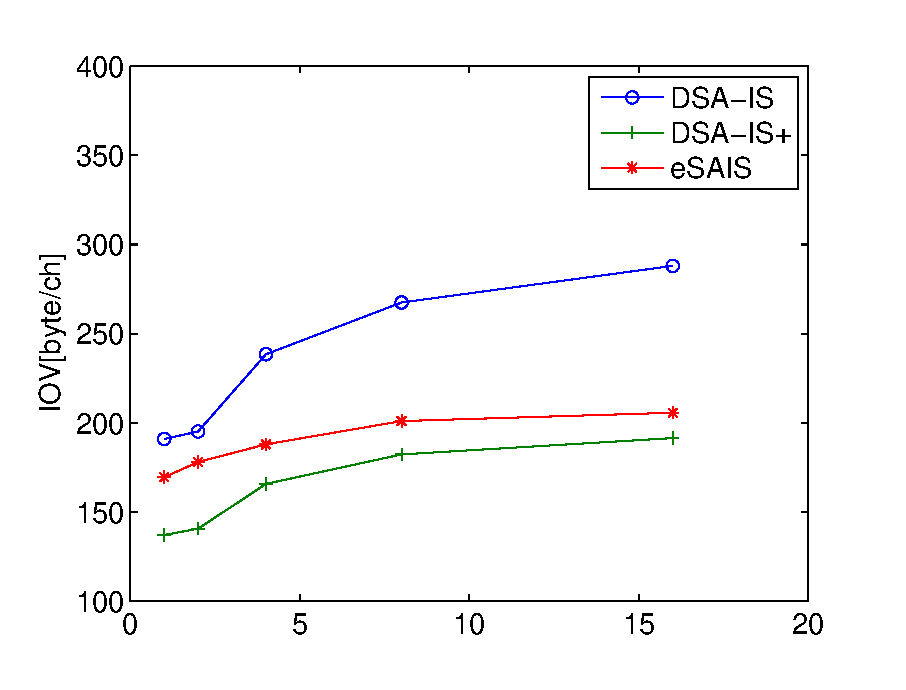
\includegraphics[width=1\textwidth]{construction_iov_enwiki} \\
			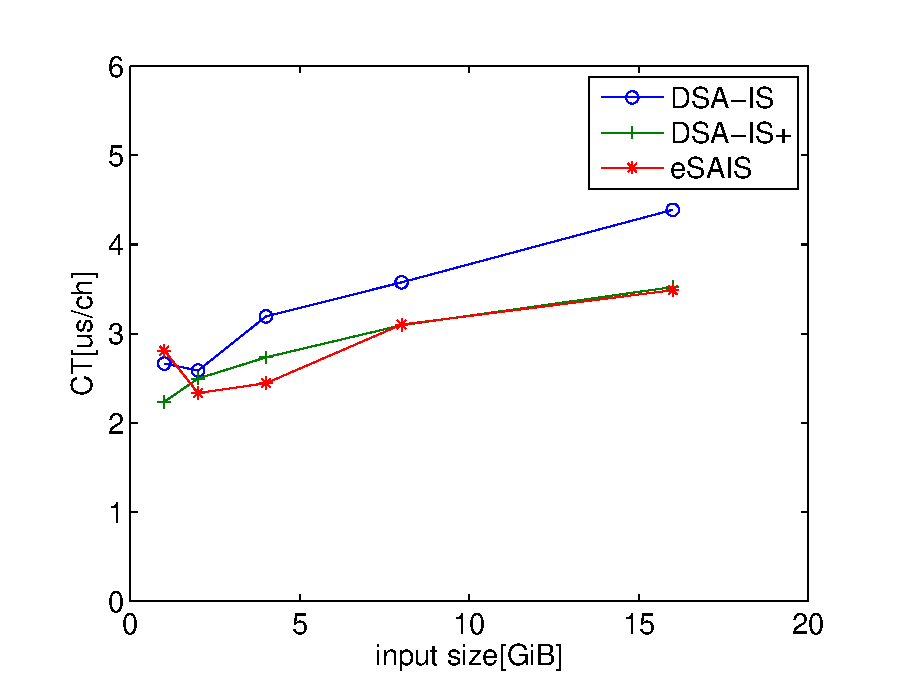
\includegraphics[width=1\textwidth]{construction_ct_enwiki}
		\end{minipage}
	}
	\subfigure[guten]{
		\begin{minipage}[b]{0.45\textwidth}
			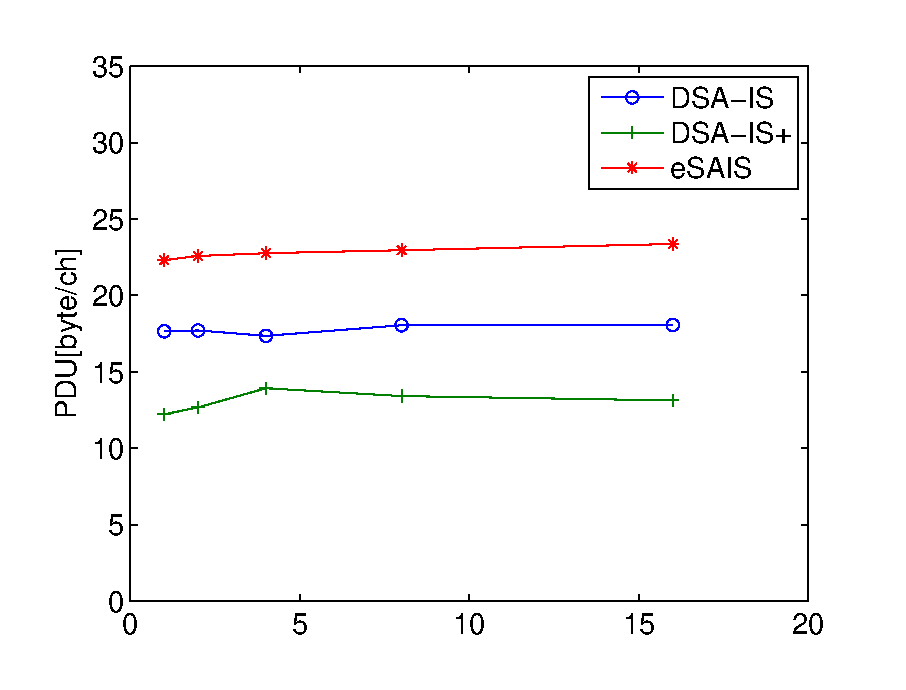
\includegraphics[width=1\textwidth]{construction_pdu_guten} \\
			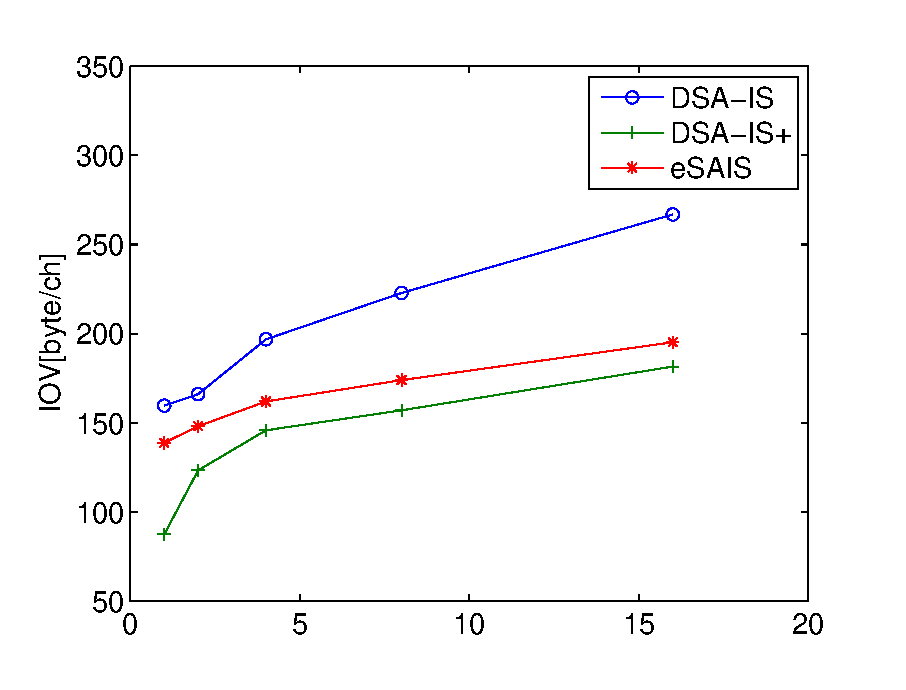
\includegraphics[width=1\textwidth]{construction_iov_guten} \\
			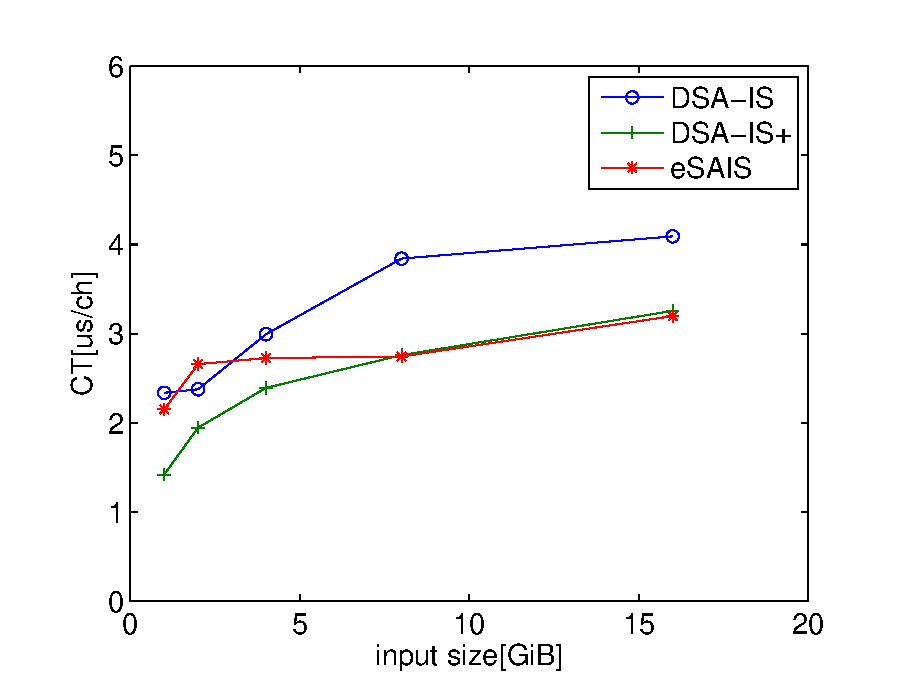
\includegraphics[width=1\textwidth]{construction_ct_guten}
		\end{minipage}
	}
	\caption{A comparison of DSA-IS, DSA-IS+ and eSAIS on guten and enwiki in terms of peak disk usage, I/O volume and construction time, where $D = 4$ and the input size varies in \{1, 2, 4, 8, 16\} GiB. }
	\label{fig:construction_performance1}
\end{figure*}

% Table
\begin{table*}%
	\caption{A Comparison of Reduction and Induction I/O Volumes Amongst DSA-IS, DSA-IS+ and eSAIS on enwiki}
	\label{tbl:volume_cmp}
	\centering
	\begin{tabular}{|c|c|c|c|c|c|c|c|c|c|c|c|c|}
		\hline
		\multicolumn{1}{|c}{} & \multicolumn{4}{|c|}{eSAIS} & \multicolumn{4}{c|}{DSA-IS} & \multicolumn{4}{c|}{DSA-IS+ ($D = 4$)}\\\hline
		\hline
		Size & Red. & Ind. & Total & Ratio & Red. & Ind. & Total & Ratio & Red. & Ind. & Total & Ratio\\\hline
		1G & 36.6 & 132.8 & 169.4 & 0.27 & 81.3 & 109.6 & 190.9 & 0.74 & 45.4 & 91.7 & 137.1 & 0.33\\\hline
		2G & 36.0 & 141.9 & 177.9 & 0.25 & 83.5 & 111.6 & 195.1 & 0.75 & 47.2 & 93.4 & 140.6 & 0.34\\\hline
		4G & 35.6 & 152.1 & 187.7 & 0.23 & 94.3 & 144.1 & 238.4 & 0.65 & 54.1 & 111.5  & 165.6 & 0.33\\\hline
		8G & 35.2 & 165.7 & 200.9 & 0.21 & 107.8 & 159.6 & 267.4 & 0.68 & 60.1 & 122.1 & 182.2 & 0.33\\\hline
		16G & 35.0 & 172.1 & 207.1 & 0.20 & 121.9 & 166.1 & 288.0 & 0.73 & 62.7 & 128.7 & 191.4 & 0.33\\\hline
	\end{tabular}
\end{table*}%

Because fSAIS is not available online, we use eSAIS as a baseline for analyzing the performance of DSA-IS and DSA-IS+. Fig.~\ref{fig:construction_performance1} shows a comparison between the programs for these three algorithms in terms of the investigated metrics. As depicted, the program for DSA-IS requires less disk space than that for eSAIS when running on "enwiki" and "guten". In details, the peak disk use of DSA-IS and eSAIS are around $18n$ and $24n$, respectively. However, eSAIS runs much faster than DSA-IS due to the different I/O volumes. In order for a deep insight, we collect in Table~\ref{tbl:volume_cmp} the statistics of their I/O volumes in the reduction and induction phases. As can be seen, although DSA-IS and eSAIS have similar performances when sorting suffixes in the induction phase, the latter consumes much less I/O volume than the former when sorting substrings in the reduction phase. More specifically, the mean ratio of induction I/O volume to reduction I/O volume are $0.23$ and $0.71$ for them, respectively. We can also see from the same figure that DSA-IS+ achieves a substantial improvement against DSA-IS, it runs as fast as eSAIS and takes half as much disk space as the latter. This is because the reduction I/O volume for DSA-IS+ is only half as much as that for DSA-IS (Table~\ref{tbl:volume_cmp}). Notice that the new substring sorting and naming methods adopted by DSA-IS+ take effect when most of the S*-type substrings are short. From our experiments, given $D = 8$, the ratio of long S*-type substrings in the investigated corpus nearly approaches one hundred percent. Therefore,the proposed substring sorting and naming methods are practical for real-world datasets.

\subsection{Checking Performance}

For evaluation, we integrate Method B into DSA-IS+ to constitute "Solution A" and compare it with "Solution B" composed of eSAIS and the existing checking method in~\cite{Dementiev2008a}. Fig.~\ref{fig:verification_performance} gives a glimpse of the performance of two solutions on various corpora. It can be observed that, the time, space and I/O volume for verification by Method B is negligible in comparison with that for construction by DSA-IS+, while the overhead for checking SA in Solution B is relatively large. Table~\ref{tbl:breakdown_solutionb} shows the performance breakdown of Solution B, where the checking time is one-fifth as the running time of the plain eSAIS and the peak disk use for verification is also a bit larger than that for construction. As a result, the combination of DSA-IS+ and Method B can build and check an SA in better total time and space.

\begin{figure}[t]
	\centering
	\subfigure{
		\label{subfig:verification_pdu}
		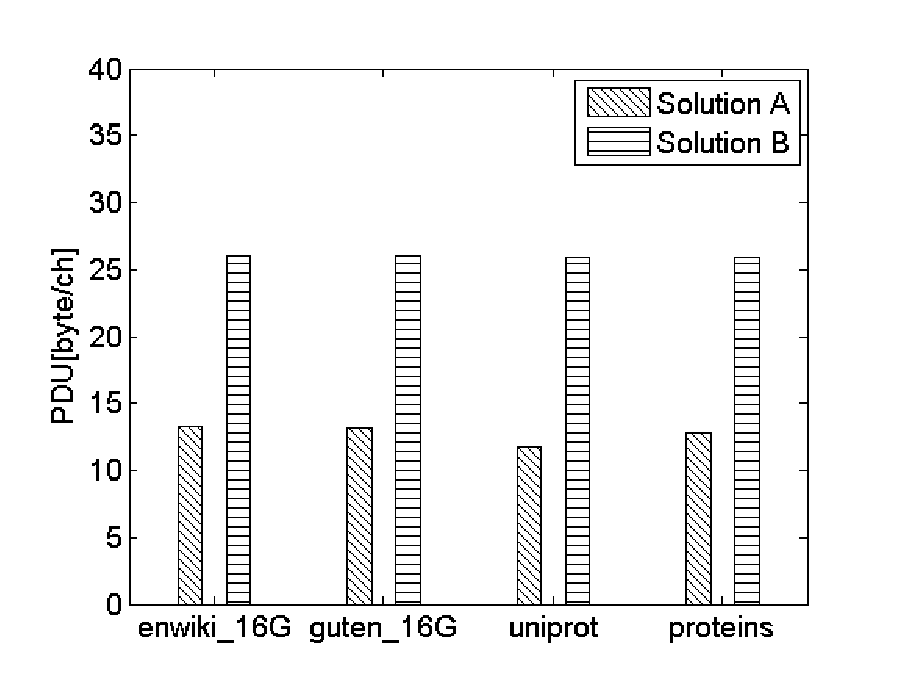
\includegraphics[width = 0.9\columnwidth]{verification_pdu}
	}
	\hfil
	\subfigure{
		\label{subfig:verification_iov}
		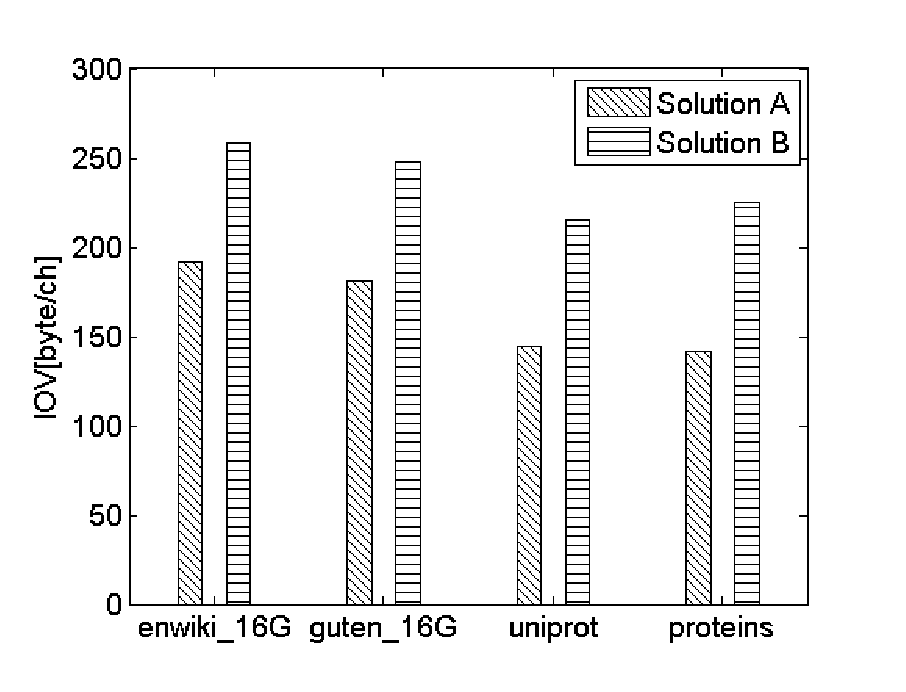
\includegraphics[width = 0.9\columnwidth]{verification_iov}
	}
	\hfil
	\subfigure{
		\label{subfig:verification_ct}
		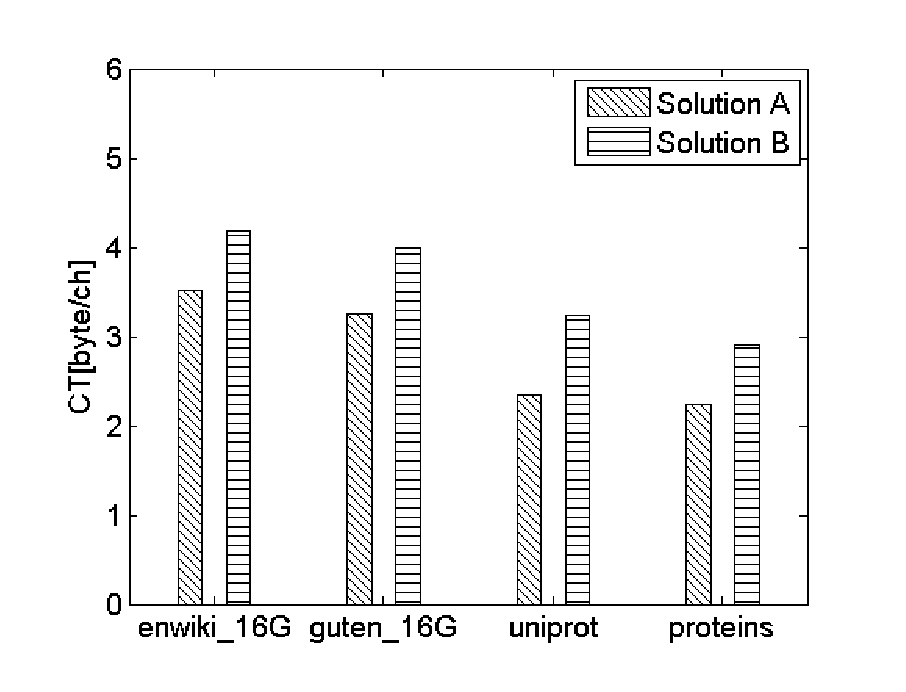
\includegraphics[width = 0.9\columnwidth]{verification_ct}
	}
	\caption{A comparison of DSA-IS and eSAIS on various corpora in terms of peak disk usage, I/O volume and construction time.}
	\label{fig:verification_performance}
\end{figure}

% Table
\begin{table}%
	\caption{Performance Breakdown of Solution B on various Corpora}
	\label{tbl:breakdown_solutionb}
	\centering
	\begin{tabular}{|c|c|c|c|c|c|c|}
		\hline
		\multirow{2}{*}{Corpus} & \multicolumn{3}{|c}{checking} & \multicolumn{3}{|c|}{building} \\\cline{2-7}
		& PDU & IOV & CT & PDU & IOV & CT \\\hline
		enwiki\_16G & 26.0 & 53.0 & 0.71 & 23.5 & 205.6 & 3.49 \\\hline
		guten\_16G & 26.0 & 53.0 & 0.79 & 23.4 & 195.2 & 3.20 \\\hline
		uniprot & 25.9 & 53.0 & 0.74 & 22.7 & 162.0 & 2.50 \\\hline
		proteins & 25.9 & 53.0 & 0.58 & 24.1 & 172.3 & 2.33 \\\hline
	\end{tabular}
\end{table}%

According to Corollary~\ref{corollary:2}, Method A must check both $sa^*$ and $sa$ to accomplish verification. Similar to Method B, the overhead for checking $sa$ is mainly caused by fingerprint calculations and thus can be neglected. On the other hand, we can apply the method proposed in~\cite{wu2017} to ensure the correctness of $sa^*$ within sorting complexity, where the time and space in need is proportional to the number of S*-type characters in $x$. Because the ratio of S*-type characters to all in $x$ is commonly one-third in real-world datasets, the checking process for $sa^*$ will not become the bottleneck for Method A. We also point out that this checking process can be parallelized with that for $sa$ to achieve a higher speed.

\section{Conclusion} \label{sec:conclusion}

In this paper, we made an attempt to improve the space performance of DSA-IS by new substring sorting and naming methods. For implementation convenience, we currently employ the STXXL's containers to perform reading, writing and sorting on the disk. The experimental results shows that our program for the adapted algorithm DSA-IS+ runs as fast as eSAIS and requires only half disk space as that for the latter on various real-world datasets. This program can be further optimized to approach the optimal space performance by means of the external-memory vector, sorter and priority queues supporting fine-grained disk space allocation and deallocation.

We also proposed two methods that enable any IS suffix sorting algorithm to build and check SA simultaneously. The second method is rather lightweight in terms of that its time and space complexities are negligible compared with that of the existing IS suffix sorting/checking algorithms. We will describe in another paper a disk-based suffix sorting algorithm taking only $1n$ work space. By augmenting with this new suffix array builder, the proposed checking methods may potentially constitute the best solution for the situations where checking is a must after building.

\bibliographystyle{IEEEtran}
\bibliography{IEEEabrv,bibfile}

\end{document}




A series of experiments are conducted to investigate the effect of $D_1$ and $D_2$ on the performance of DSA-IS+. As shown in Figure~\ref{fig:performance_analysis3}, the time consumption of DSA-IS+ gets smaller as $D_2$ becomes larger, while the peak disk usage and I/O volume are almost unchanged. Furthermore, the data of Table~\ref{tbl:effect_of_D} indicates that a small variation on the values of $D_1$ and $D_2$ can incur a significant fluctuation on the speed of DSA-IS+. For instance, when changing $(D_1, D_2)$ from $(8, 10)$ to $(16, 16)$, the construction time for the uniprot dataset decreases from 2.64 to 2.24 microseconds per character. This is because the proportions of long LMS substrings of $x$ and $\{x1, x2,...\}$ decrease when $D_1$ and $D_2$ increase. Recall that, after partitioning $x$ into blocks, DSA-IS+ sorts the long LMS substrings of each block in RAM and merges them by an external memory sorter, which is time-consuming when the number of long LMS substrings is large. In our program, the ratio of long and short LMS substrings can be controlled by adjusting the values of $D_1$ and $D_2$. However, when $D_1$ and $D_2$ get larger, the min heap also takes more time to merge the sorted short and long LMS substrings, as each string comparison takes $\mathcal{O}(D_1)$ and $\mathcal{O}(D_2)$ time in the first and recursion levels, respectively. Fortunately, Table~\ref{tbl:long_short_distribution} shows that the majority of LMS substrings in real datasets are considerably short. In practice, we can set $D_1$ and $D_2$ according to the statistics of the length distribution of LMS substrings, where the statistics can be collected when partitioning $x$ at the beginning of the reduction phase.

\begin{table*}[htbp]
	\caption{Effects of $D_1$ and $D_2$ for DSA-IS+}
	\label{tbl:effect_of_D}
	\centering
	\begin{tabular}{|c|c|c|c|c|c|c|c|c||c|c|c|c|c|}
		\hline
		\multicolumn{1}{|c}{} & \multicolumn{3}{|c}{eSAIS} & \multicolumn{10}{|c|}{DSA-IS+}\\\hline
		\hline
		Corpora & PDU & IOV & CT & $D_1$ & $D_2$ & PDU & IOV & CT  & $D_1$ & $D_2$ & PDU & IOV & CT\\\hline
		uniprot & 22.71 & 162.01 & 2.50 & 8 & 10 & 14.27 & 146.10 & 2.64 & 16 & 16 & 14.27 & 144.90 & 2.24 \\\hline
		proteins & 24.09 & 172.29 & 2.33 & 8 & 10 & 16.12 & 147.92 & 2.28 & 20 & 12 & 16.12 & 147.85 & 2.14 \\\hline
		genome & 22.64 & 157.41 & 2.15 & 8 & 10 & 15.34 & 142.05 & 2.75 & 20 & 12 & 15.34 & 140.89 & 2.25 \\\hline
	\end{tabular}
\end{table*}%

\begin{figure}[htbp]
	\centering
	\subfigure{
		\centering
		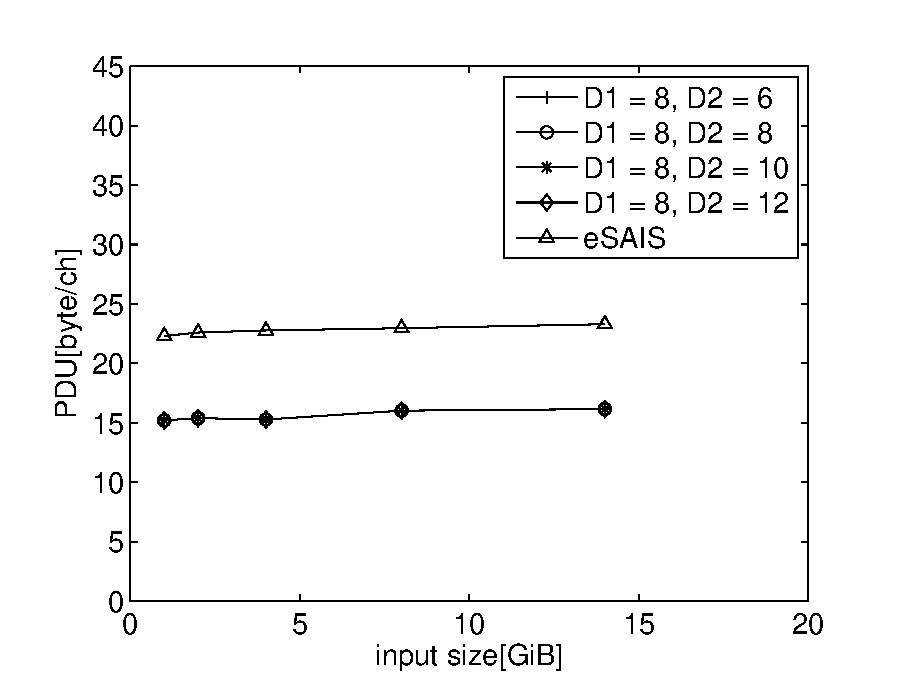
\includegraphics[width=0.9\columnwidth]{pdu_cmp3}
		\label{subfig:pdu_cmp3}
	}
	\hfil
	\subfigure{
		\centering
		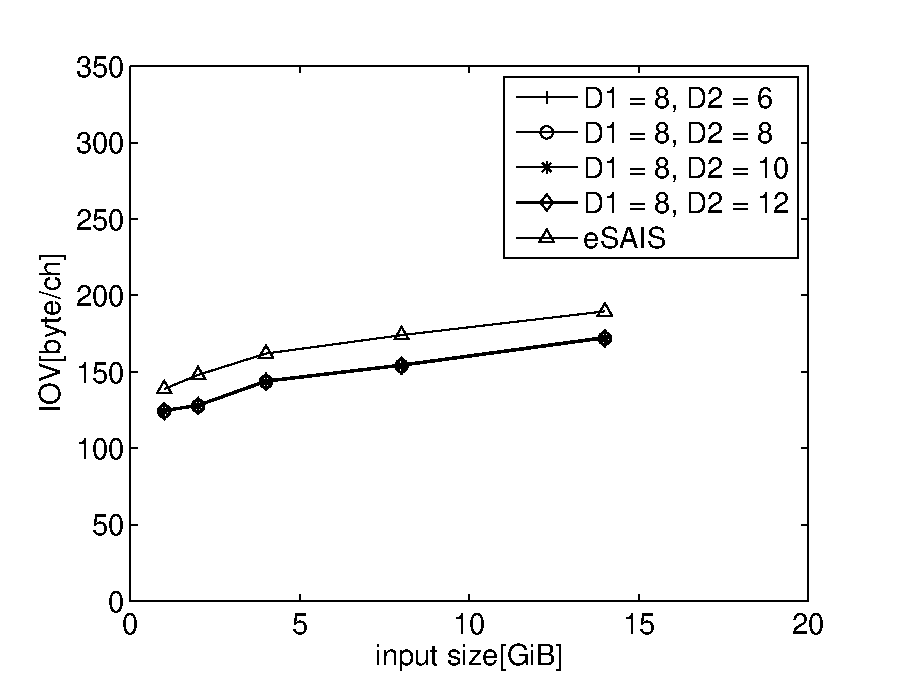
\includegraphics[width=0.9\columnwidth]{iov_cmp3}
		\label{subfig:iov_cmp3}
	}
	\hfil
	\subfigure{
		\centering
		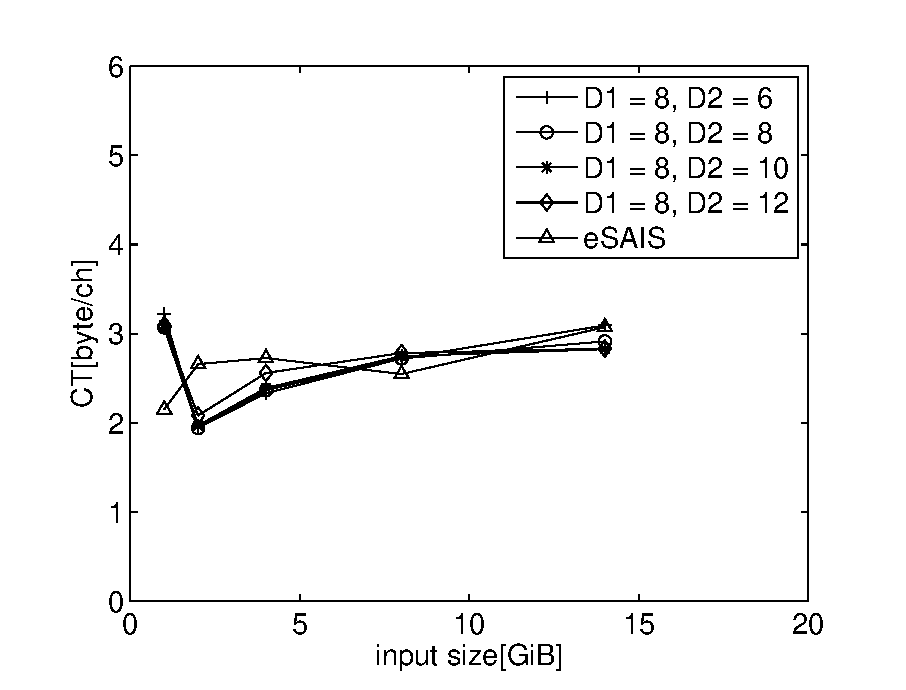
\includegraphics[width=0.9\columnwidth]{ct_cmp3}
		\label{subfig:ct_cmp3}
	}
	\caption{Experimental results for DSA-IS+ and eSAIS on guten in terms of peak disk usage, I/O volume and construction time, where $D_1 = 8$, $D_2$ ranges in \{6, 8, 10, 12\} and the input size varies in \{1, 2, 4, 8, 14\} GiB. }
	\label{fig:performance_analysis3}
\end{figure}


\begin{table*}[htbp]
	\caption{Statistics on the Length Distribution of Long and Short LMS Substrings for DSA-IS+}
	\label{tbl:long_short_distribution}	
	\centering
	\begin{tabular}{|c|c|c|c|c|c|c|c|c|c|c|}
		\hline
		\multicolumn{11}{|c|}{level 0} \\\hline
		Corpora & $D_1$ & long & short & total & ratio & $D_1$ & long & short & total & ratio\\\hline
		uniprot & 8 & 30243605 & 785997413 & 816241018 & 0.963 & 16 & 3850755 & 812390263 & 816241018 & 0.999\\\hline
		proteins & 8 & 1687673 & 377404329 & 379092002 & 0.999 & 20 & 10930 & 379081072 & 379092002 & 0.999\\\hline
		genome & 8 & 19446841 & 773670266 & 793117107 & 0.975 & 20 & 509998 & 792607109 & 793117107 & 0.999\\\hline
		\multicolumn{11}{|c|}{level 1}\\\hline
		Corpora & $D_2$ & long & short & total & ratio & $D_2$ & long & short & total & ratio\\\hline
		uniprot & 10 & 11849 & 263748775 & 263760624 & 0.995 & 16 & 380 & 263760244 & 263760624 & 0.999\\\hline
		proteins & 10 & 18126 & 123772731 & 123790857 & 0.996 & 20 & 2937 & 123787920 & 123790857 & 0.999\\\hline
		genome & 10 & 311607 & 248243216 & 248554823 & 0.999 & 20 & 153845 & 248400978 & 248554823 & 0.999\\\hline
	\end{tabular}
\end{table*}%


\subsection{Checking Performance}

\begin{table*}[htbp]
	\caption{Overall Performance of DSA-IS+ and eSAIS with CM1 and CM2 on enwiki\_8G}
	\label{tbl:check_overhead}
	\centering
	\begin{tabular}{|c|c|c|c|c|c|c|}
		\hline
		& \multicolumn{3}{|c|}{DSA-IS+ ($D_1 = 8$, $D_2 = 10$)} & \multicolumn{3}{c|}{eSAIS}\\\hline
		Checking Method & PDU & IOV & CT & PDU & IOV & CT \\\hline
		CM1 & 17.93  & 180.01 & 3.10 & - & - & - \\\hline
		CM2 & 26.00 & 231.68 & 4.00 & 27.00 & 246.93 & 3.74 \\\hline
		no check & 17.93  & 173.67	& 3.17 & 23.85 & 200.93 & 3.10 \\\hline
	\end{tabular}
\end{table*}%


We make a performance comparison of the proposed checking method and the work presented in~\cite{Karkkainen2003}, which are denoted by CM1 and CM2, respectively. For performance evaluation, we integrate CM1 into the program of DSA-IS+ following Section~\ref{subsec:sachecker:implementation} and reuse the implementation for CM2 in the program of eSAIS to verify the outputs of DSA-IS+ and eSAIS. Table~\ref{tbl:check_overhead} gives a glimpse of the performance overhead for the two checking methods. It can be seen that, when checking the suffix array of enwiki\_8G by using CM2, both time and I/O volume for verification are about one-fifth of that for construction. On the other hand, CM1 has almost no negative impact on the overall performance. As demonstrated in lines 3 and 5, the peak disk usage for CM1 is no more than that for DSA-IS+ and the increase in the I/O volume can be ignored. It worth mentioning that the data of the running time for the combination of DSA-IS+ and CM1 is a bit shorter than that for the plain DSA-IS+. This is a normal phenomenon due to the fluctuating I/O performance, which in turn indicates that the time overhead consumed by CM1 is also negligible.

